\section{Five Parameter Solar Cell Model}\label{sec:five_parameter_solar_cell_model}

\subsection{Model Introduction}\label{subsec:five_param_model_introduction}

\begin{figure}[h]
    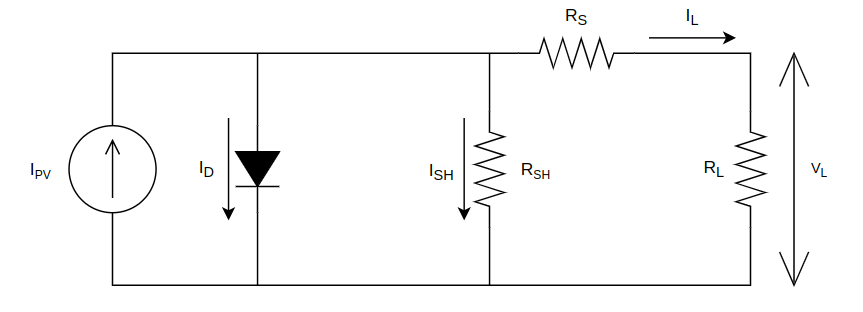
\includegraphics[width=\textwidth]{solar_cell_five_parameter_model.png}
    \caption{Five Parameter, or Full Single Diode Model of a Solar Cell}
    \label{fig:single_diode_model_with_resistances}
\end{figure}

The most common model for solar cells is the five parameter solar cell model,
shown in Figure~\ref{fig:single_diode_model_with_resistances}. This is the
complete form of the single diode model discussed in the previous section,
Section~\ref{sec:three_parameter_solar_cell_model}. There are two added
components/parameters: a series resistance \ac{RS} and shunt resistance
\ac{RSH}, whose primary roles are to alter the shape of the knee-bend in the I-V
curve. As such, this model improves upon the main flaw of the three parameter
solar cell model, that of overshooting the maximum power point.

In the following subsections, we discuss the two added parameters and their
specific effects on the model.


\subsection{Shunt Resistance}\label{subsec:five_param_shunt_resistance}

\begin{figure}[h]
    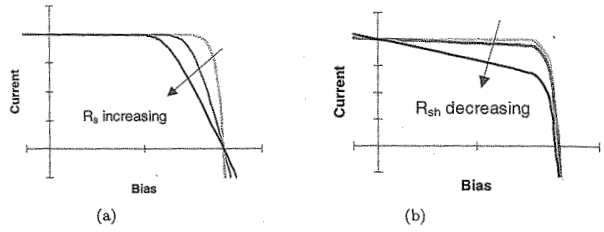
\includegraphics[width=\textwidth]{series_shunt_resistance.png}
    \caption{Effect of Series (a) and Shunt Resistance (b) on \ac{I-V} Curve}
    \label{fig:series_shunt_resistance}
\end{figure}

As shown in Figure~\ref{fig:series_shunt_resistance} (b) from
Nelson~\cite{nelson}, as the shunt resistance \ac{RSH} decreases, the top of the
knee-bend of the \ac{I-V} curve will be forced down. At low values of shunt
resistance (on the order of $10$ $\si{\ohm}$), the knee-bend will be pushed down
so much that the curve becomes a straight line. At high values of shunt
resistance, (on the order of $100$ $\si{\ohm}$), the curve converges to some
fixed maximum bend constrained by other parameters of the model. This
relationship is generally considered logarithmic.

The \ac{ISH} can be added to the simple form of the model as a new term as shown
in Equation~\ref{eq:cell_output_current_3}. Assuming that the series resistance
is negligible ($0$), we can determine that \ac{ISH} is a function of the
\ac{RSH} and the voltage across the cell \ac{VL}, as shown in
Equation~\ref{eq:cell_output_current_4}.

\begin{equation}
    I_L = I_{PV} - I_D - I_{SH}
    \equnit{\si{\ampere}}
    \label{eq:cell_output_current_3}
\end{equation}

\begin{equation}
    I_L = I_{PV} - I_D - \frac{V_L}{R_{SH}}
    \equnit{\si{\ampere}}
    \label{eq:cell_output_current_4}
\end{equation}


\subsection{Series Resistance}\label{subsec:five_param_series_resistance}

The series resistance \ac{RS} forces the knee-bend of the \ac{I-V} curve to the
left or right, as opposed to up and down for the shunt resistance. As the series
resistance increases, more current is consumed across the lumped resistance
before reaching the terminals of the solar cell, reducing the expected current
in the curve as shown in Figure~\ref{fig:series_shunt_resistance} (a). At high
values of series resistance, the curve likewise becomes a straight line.

The series resistance \ac{RS} term impacts the consumers of the five parameter
solar cell model; namely the dark current and the shunt resistance terms. A
visualization of this is shown as Figure~\ref{fig:current_junction}.

\begin{figure}[h]
    \centering
    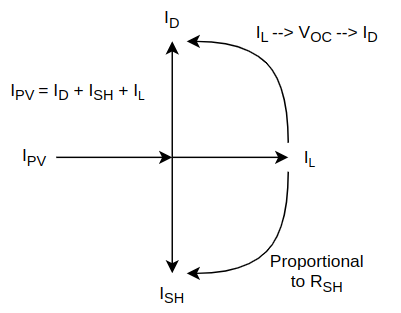
\includegraphics[width=0.7\textwidth]{cell_kirchoff_current_junction.png}
    \caption{Current Flow Junction of Five Parameter Model Solar Cell}
    \label{fig:current_junction}
\end{figure}

Revisiting Equation~\ref{eq:cell_dark_current_1}, we know that the dark current
depends on the voltage across the cell \ac{VL} generated by the load current
\ac{IL} flowing through the load resistance \ac{RL} connected at the cell
terminals. This allows us to reformulate the dark current equation as
Equation~\ref{eq:cell_dark_current_2}. Here, we add the voltage drop across the
lumped series resistance summed with the load voltage \ac{VL} to represent the
total voltage expected by the dark current model.

\begin{equation}
    I_D = I_0[\exp(\frac{V_L + I_L R_S}{V_T}) - 1]
    \equnit{\si{\ampere}}
    \label{eq:cell_dark_current_2}
\end{equation}

We can likewise use the voltage drop to update the shunt resistance term, shown
in Equation~\ref{eq:cell_shunt_current}.

\begin{equation}
    I_{SH} = \frac{V_L + I_L R_S}{R_{SH}}
    \equnit{\si{\ampere}}
    \label{eq:cell_shunt_current}
\end{equation}

Combining these two effects, we form Equation~\ref{eq:cell_output_current_5}.

\begin{equation}
    I_{L} =  I_{PV} - I_0[\exp(\frac{V_L + I_L R_S}{V_T}) - 1] - \frac{V_L + I_L R_S}{R_{SH}}
    \equnit{\si{\ampere}}
    \label{eq:cell_output_current_5}
\end{equation}

We note that this model is an implicit function and cannot easily (or prettily)
move all the \ac{IL} terms to the left side of the equation. As such, for these
types of problems, we will develop and use iterative solvers to determine
\ac{IL} for a given set of input parameters (\ac{RS}, \ac{G}, \ac{VL}, etc).
Iterative solvers involve starting with a guess for the output parameter (in
this case \ac{IL}) and attempt to improve upon that guess such that each side is
equal to each other or within some tolerance to each other. An in depth
discussion on how these solvers were implemented for this model and variants of
this model can be found in Appendix~\ref{appendix:iterative_solvers}.


\subsection{Photocurrent as a Ratio of Shunt/Series Resistance}\label{subsec:photocurrent_shunt_series_relation}

An interesting addition to the five parameter cell model is presented by Cubas
et al~\cite{cubas_et_al}\cite{cubas_et_al_2}: they observe that
Equation~\ref{eq:cell_output_current_5} in short circuit conditions results in
Equation~\ref{eq:cell_short_circuit_current_6}.

\begin{equation}
    I_{SC} = I_{PV} - I_0[\exp(\frac{I_{SC} R_S}{V_T}) - 1] - \frac{I_{SC} R_S}{R_{SH}}
    \equnit{\si{\ampere}}
    \label{eq:cell_short_circuit_current_6}
\end{equation}

In their analysis of measurements taken across a broad spectrum of reference
solar cells, represented in Table~\ref{table:dark_current_reference}, the dark
current at short circuit conditions were well less than a single milliampere, an
insignificant fraction of the total operating current. From this observation
Cubas et al. rewrites the above expression to get the photocurrent as a function
of the short circuit current and a ratio of the series and shunt resistance,
shown in Equation~\ref{eq:cell_photocurrent_3}.

\begin{equation}
    I_{PV} = I_{SC}\frac{R_S + R_{SH}}{R_{SH}}
    \equnit{\si{\ampere}}
    \label{eq:cell_photocurrent_3}
\end{equation}

\begin{table}[h!]
    \begin{tabularx}{\textwidth}{
        | >{\raggedright\arraybackslash}X
        | >{\raggedright\arraybackslash}X
        | >{\raggedright\arraybackslash}X
        | >{\raggedright\arraybackslash}X
        | >{\raggedright\arraybackslash}X | }
        \hline
        Reference & Cell Type & \ac{ISC} (A) & $I_0[e^{\frac{I_{SC} R_S}{V_T}} -
        1]$ (A) & \ac{ID} / \ac{ISC} \\ \hline \hline
        Kennerud, 1969  & CdS   & 0.8040 & 1.56E-5 & 1.94E-5 \\ \hline
        Charles, 1981   & BSC   & 0.1023 & 2.21E-8 & 2.16E-7 \\ \hline
        Charles, 1981   & GSC   & 0.5610 & 1.01E-5 & 1.80E-5 \\ \hline
        Lo Brano, 2010  & Q6LM  & 7.6650 & 1.42E-9 & 1.85E-10 \\ \hline
    \end{tabularx}
    \caption{Dark Current Ratios for Various Reference Cells}
    \label{table:dark_current_reference}
\end{table}

However, a cursory evaluation of the parameter space (\ac{VOC}, \ac{ISC},
\ac{G}, \ac{TC}, \ac{RS}, \ac{N}) reveals that the assumption that the dark
current is negligible breaks down when a subset of the following conditions
occur:

\begin{itemize}
    \item the open circuit voltage \ac{VOC} becomes very small,
    \item the short circuit current \ac{ISC} becomes very large,
    \item and the series resistance \ac{RS} becomes relatively large for some
    combination of \ac{VOC} and \ac{ISC}.
\end{itemize}

Is it to be noted that these parameters are tightly coupled, and therefore the
language specifying a parameter space upon which this term should be used
remains imprecise. We also note that the temperature and ideality factor
when increased slightly tighten the viable parameter space.

However, when considering a specific solar cell that is \textit{appropriate}
(e.g.\ it contains \ac{STC} defined parameters \ac{VOC} and \ac{ISC} with an
measured \ac{RS} that results negligible \ac{ID}), this term remains negligible
unless the cell is exposed to (1) high temperatures or (2) high intensity
light, two conditions that tend to come hand in hand. These conditions tend to
only be experienced by concentrator photovoltaics and are highly unlikely to be
reached by normal solar cells.

We will observe later in Section~\ref{sec:evaluation_of_solar_module_models}
that with our dataset of Maxeon Gen III Bin Le1 solar cells, the vast majority
of estimated series resistance is well below $0.08 \si{\ohm}$, which results in
dark currents less than a m\si{\ampere}. This means that this modification
(assuming it improves the accuracy of the model), is well suited for our solar
cells.

Incorporating this revision, we arrive at
Equation~\ref{eq:cell_short_circuit_current_7}.

\begin{equation}
    I_L = I_{SC}\frac{R_S + R_{SH}}{R_{SH}} - I_0[\exp(\frac{V_L + I_L R_S}{V_T}) - 1] - \frac{V_L + I_L R_S}{R_{SH}}
    \equnit{\si{\ampere}}
    \label{eq:cell_short_circuit_current_7}
\end{equation}

\todo[inline]{See \url{https://www.desmos.com/calculator/nniw0mha2k} to play
around with the revised dark current model. Add as a figure later on compared to
experimental data.}


\subsection{Shunt and Series Resistance as a Function of Irradiance, Temperature}\label{subsec:rsh_rs_dependence}

Throughout this major section, we introduced the notion of shunt and series
resistance as internal parasitics. However, we did not explore whether these
`internal parameters` are themselves affected by external conditions such as
irradiance and temperature.

A comprehensive review and experimental paper from Fébba et
al~\cite{febba_et_al} performed experiments on solar cells to evaluate the
effect of temperature and irradiance on shunt and series resistance, controlling
for the two independent variables in ranges of $25\si{\celsius}$ to
$55\si{\celsius}$ and $600\si{\watt/\meter^2}$ to $1000\si{\watt/\meter^2}$,
respectively. Four figures,
Figures~\ref{fig:febba_shunt_resistance_and_temperature}~-~\ref{fig:febba_series_resistance_and_irradiance}
are shown below to illustrate the following assertions.

For shunt resistance, they observed the following trends:

\begin{itemize}
    \item as temperature increases, the shunt resistance exponentially decays,
    \item and as irradiance increases, the shunt resistance linearly decreases.
\end{itemize}

For series resistance, they observed the following trends:

\begin{itemize}
    \item as temperature increases, the series resistance exponentially decays,
    \item and as irradiance increases, the series resistance linearly increases.
\end{itemize}

\begin{figure}[!htbp]
    \centering
    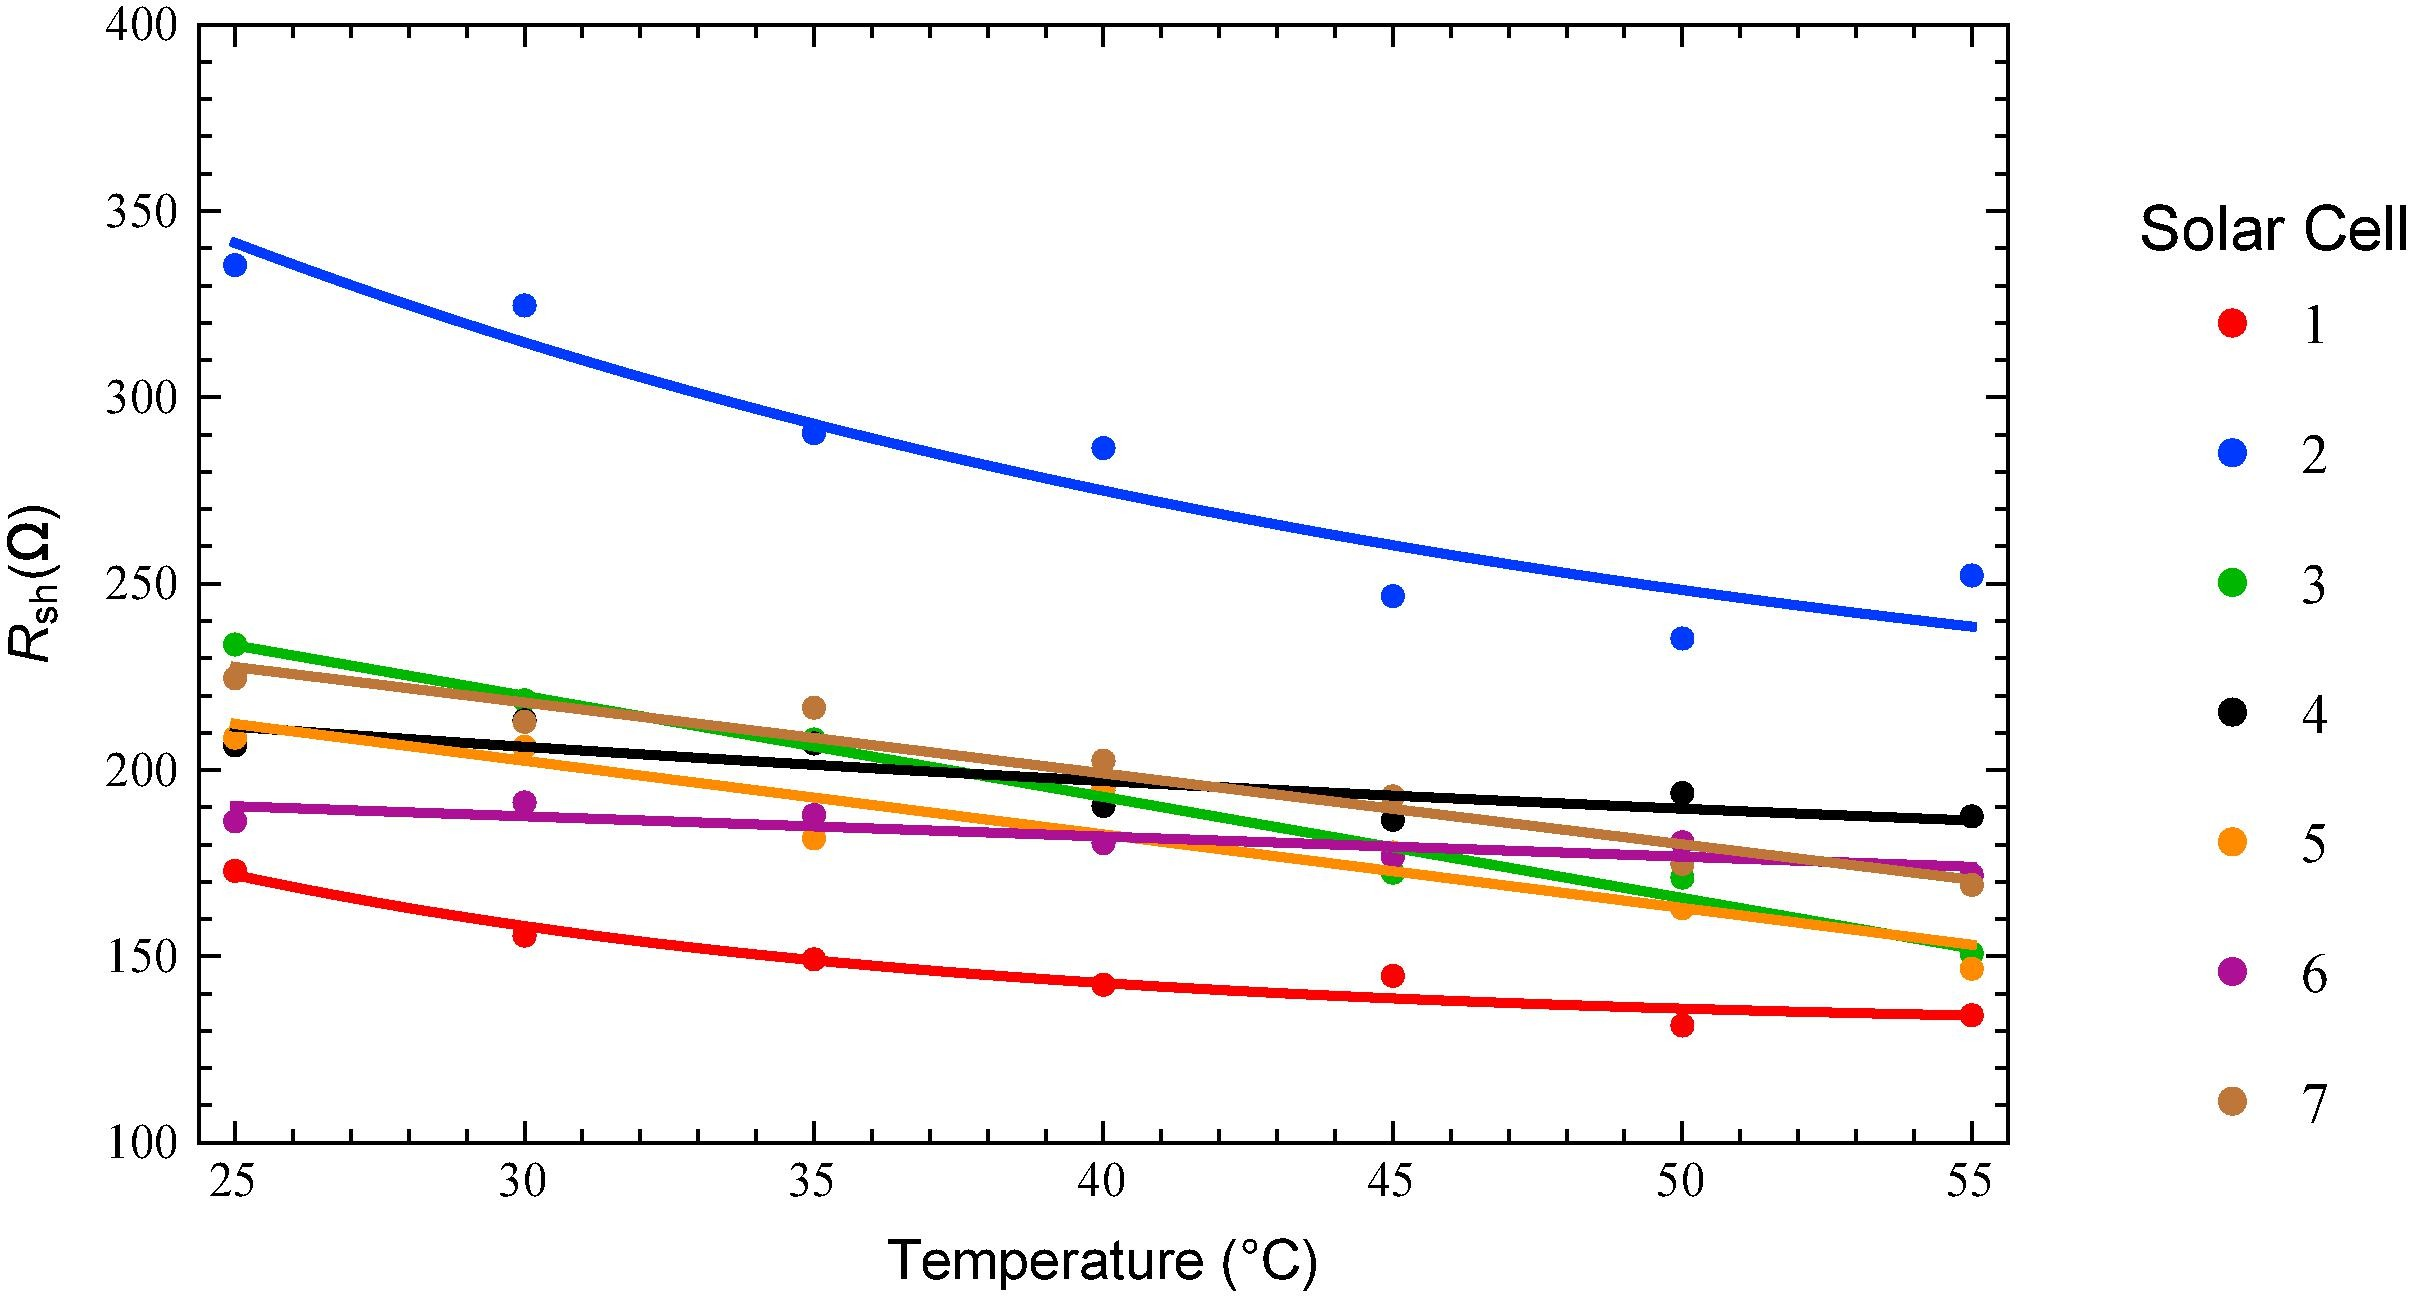
\includegraphics[width=0.75\textwidth]{febba_shunt_resistance_and_temperature.jpg}
    \caption{Shunt Resistance vs Temperature~\cite{febba_et_al}}
    \label{fig:febba_shunt_resistance_and_temperature}
\end{figure}

\begin{figure}[!htbp]
    \centering
    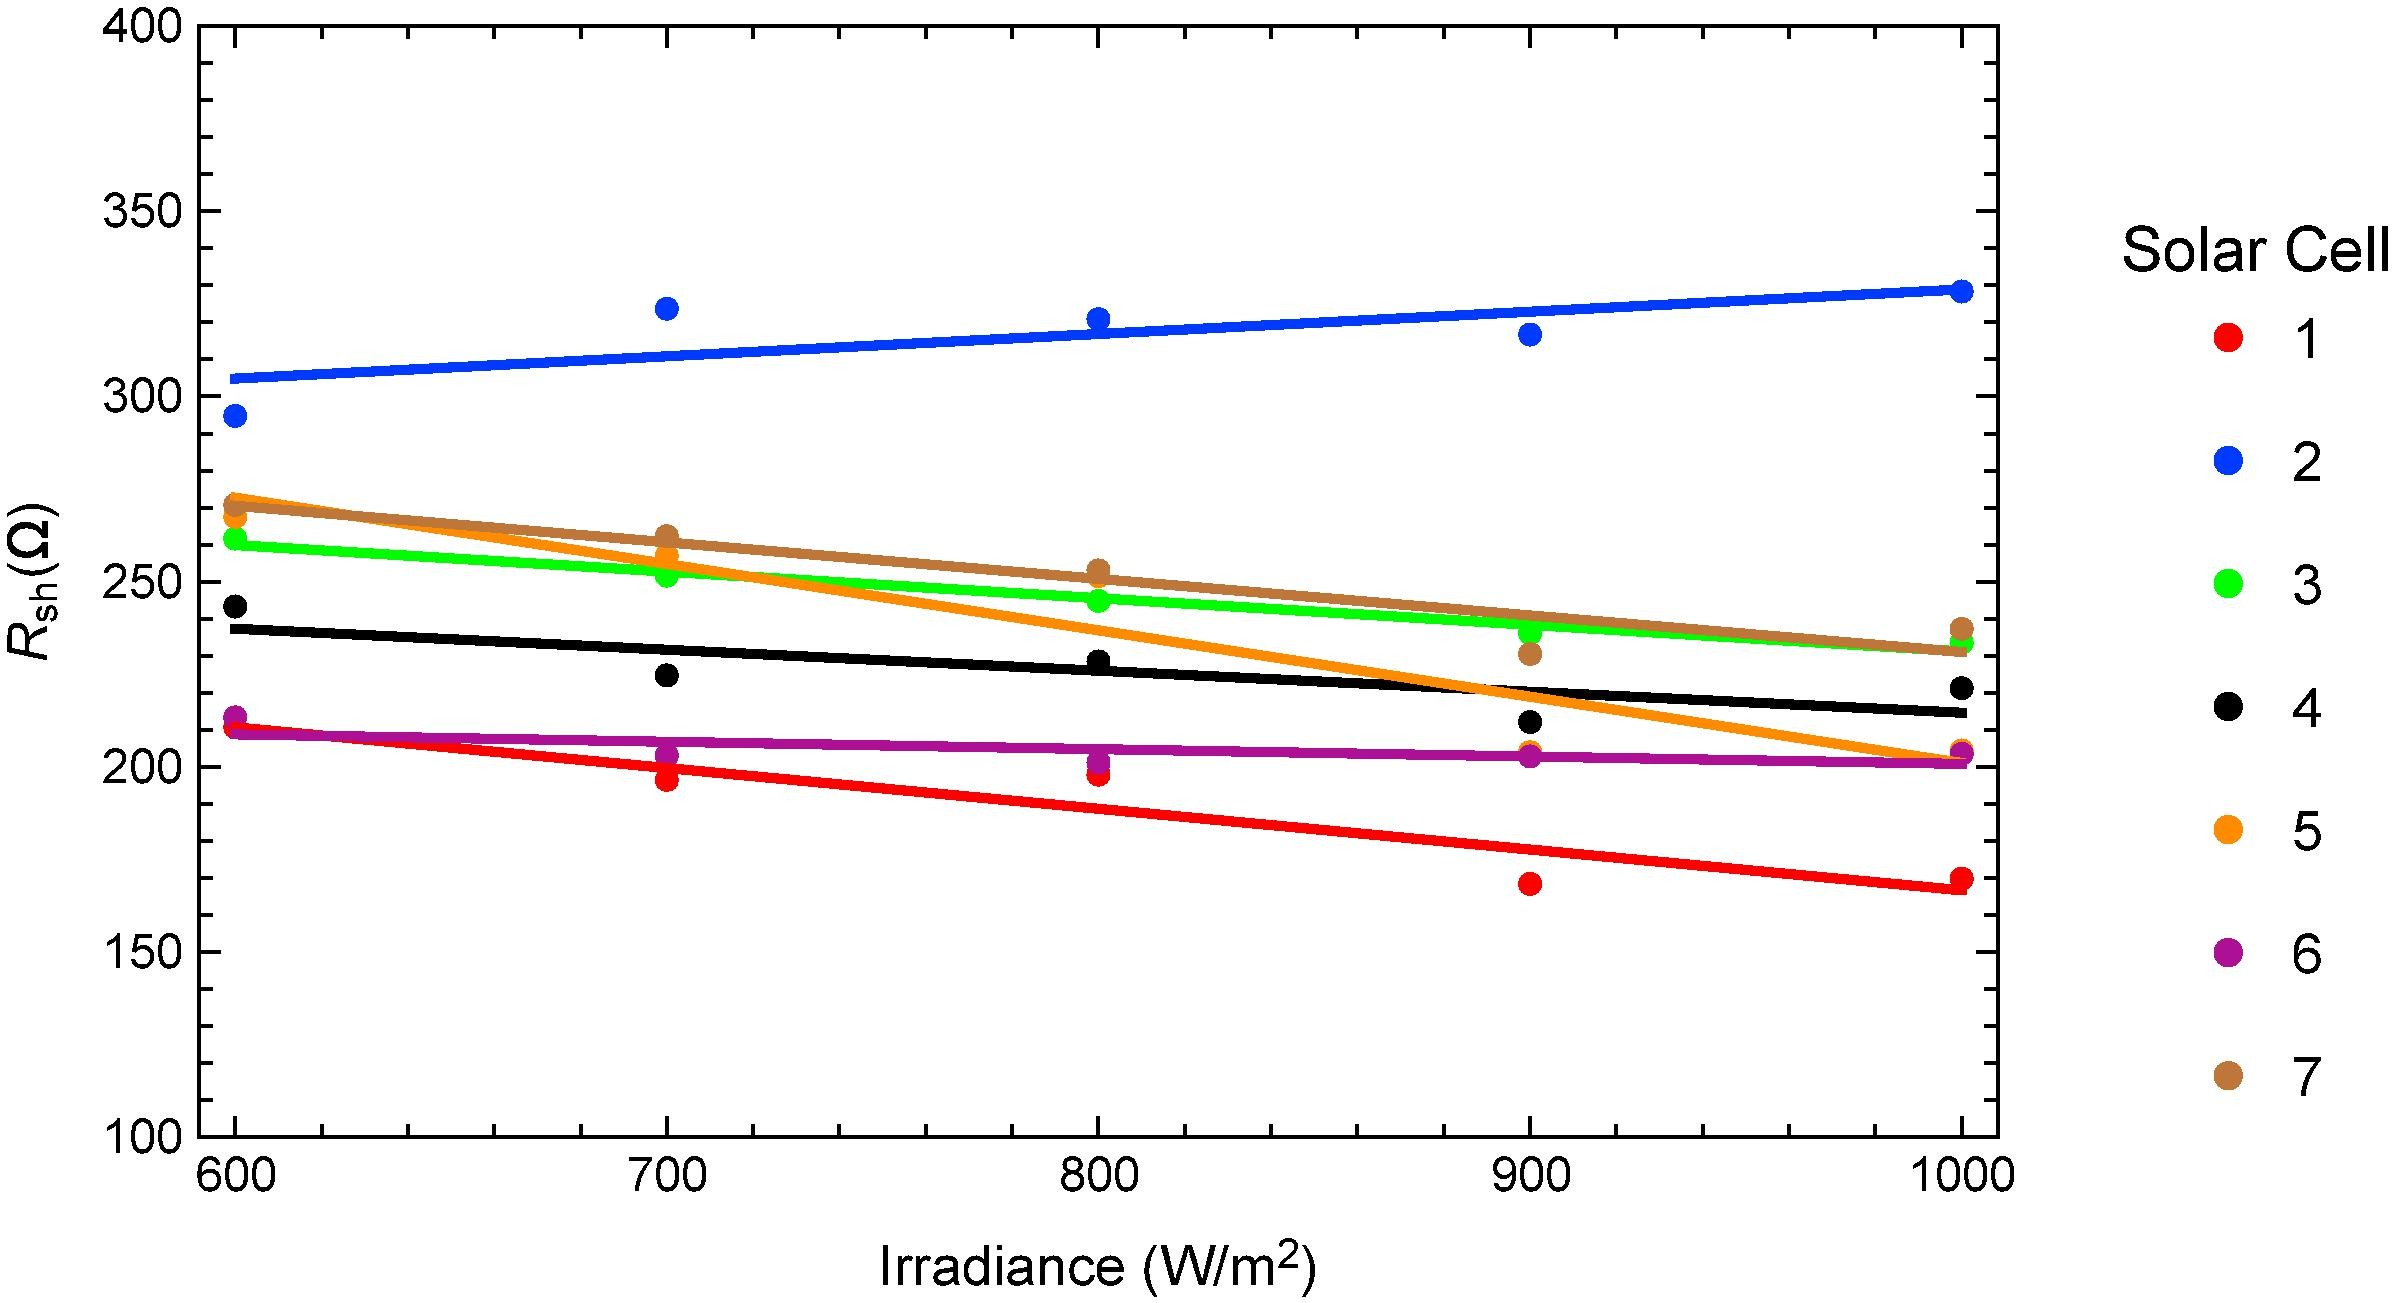
\includegraphics[width=0.75\textwidth]{febba_shunt_resistance_and_irradiance.jpg}
    \caption{Shunt Resistance vs Irradiance~\cite{febba_et_al}}
    \label{fig:febba_shunt_resistance_and_irradiance}
\end{figure}

\begin{figure}[!htbp]
    \centering
    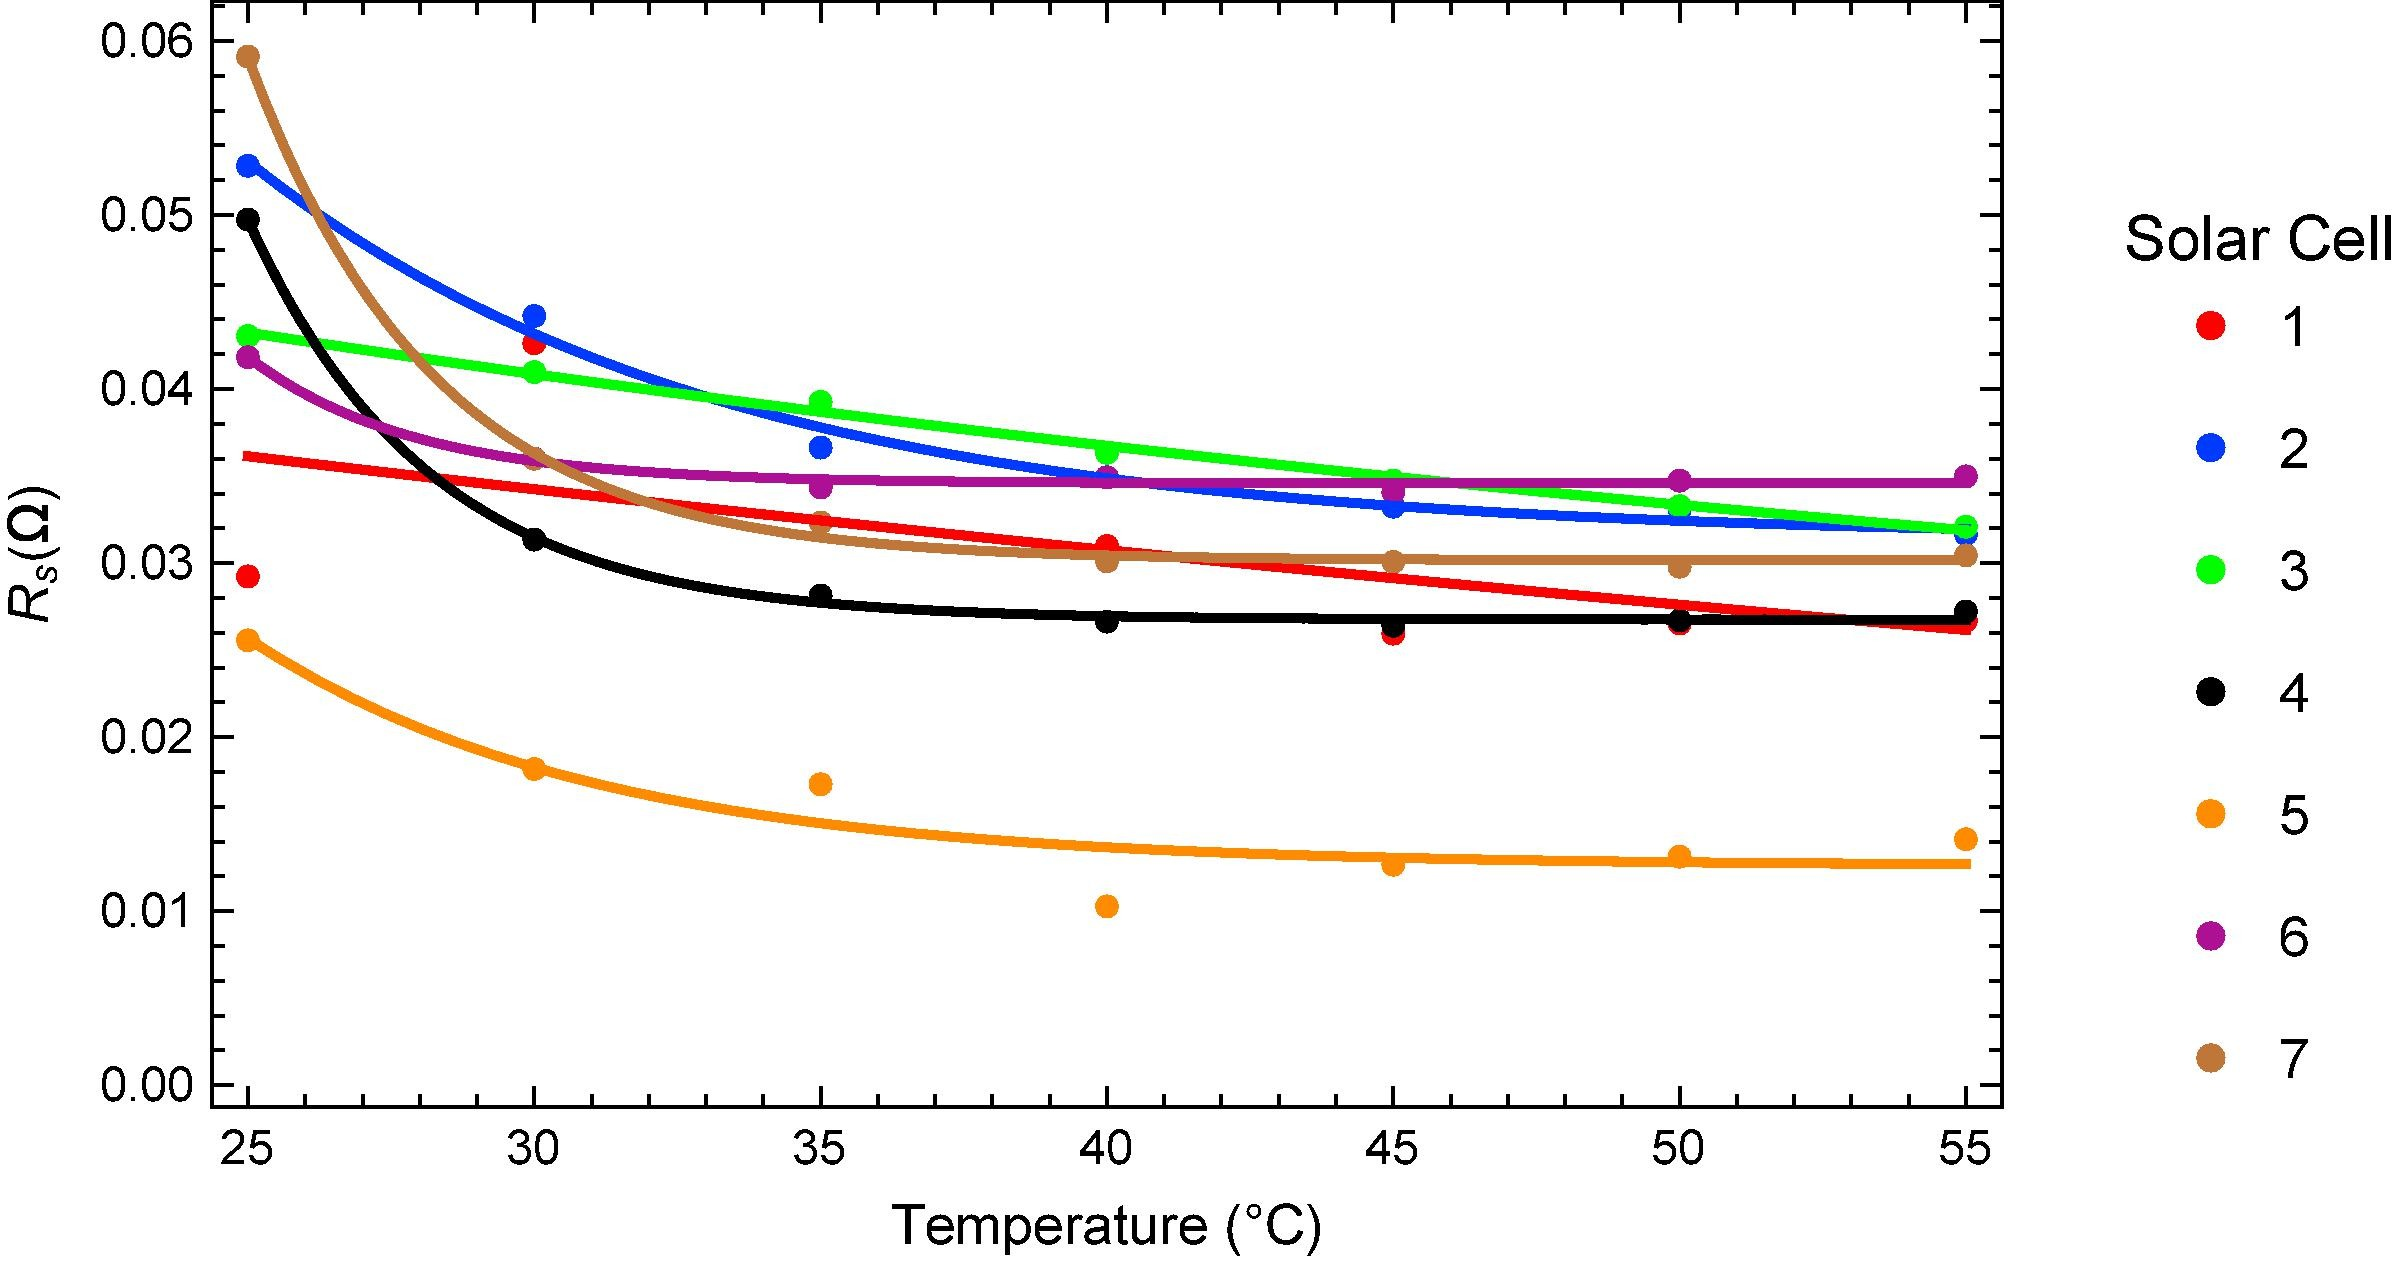
\includegraphics[width=0.75\textwidth]{febba_series_resistance_and_temperature.jpg}
    \caption{Series Resistance vs Temperature~\cite{febba_et_al}}
    \label{fig:febba_series_resistance_and_temperature}
\end{figure}

\begin{figure}[!htbp]
    \centering
    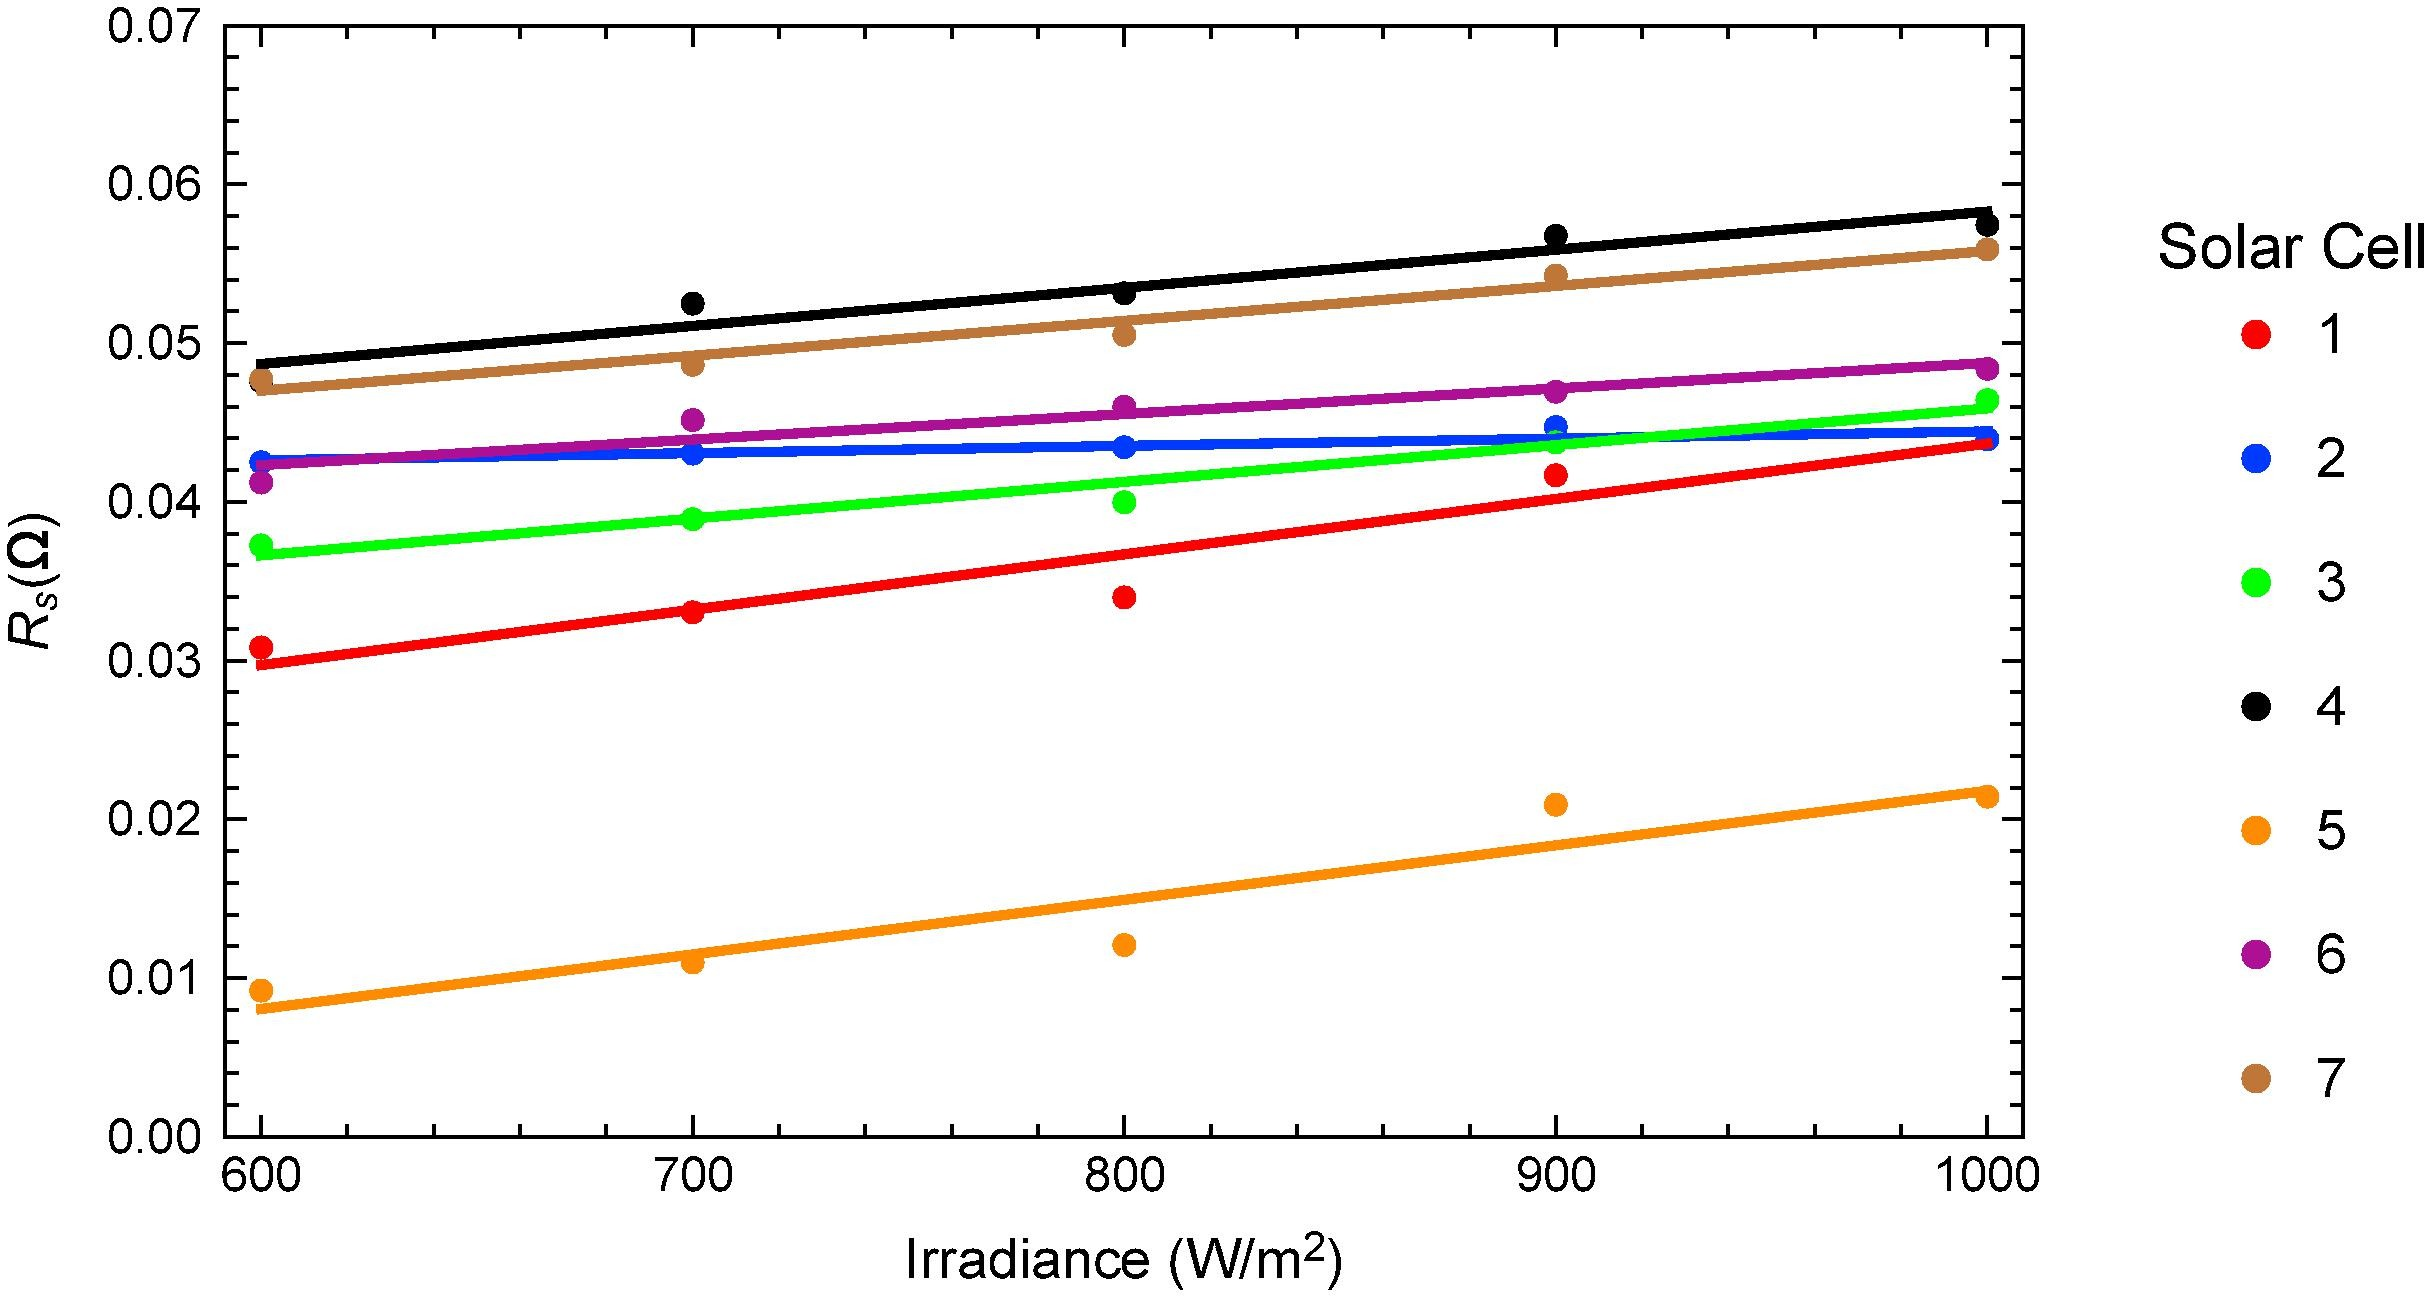
\includegraphics[width=0.75\textwidth]{febba_series_resistance_and_irradiance.jpg}
    \caption{Series Resistance vs Irradiance~\cite{febba_et_al}}
    \label{fig:febba_series_resistance_and_irradiance}
\end{figure}

Fébba et al. did not posit a revised model of the either resistance term
(although they did provide explanations on why the trends were reasonable), but
Baig et al.~\cite{baig_et_al} and MacAlpine et
Brandemuehl~\cite{macalpine_et_brandemuehl} introduced a variant of
Equation~\ref{eq:series_resistance_1}, where $\si{\zeta}$ is a new temperature
coefficient.

\begin{equation}
    R_S = R_{S,ref} \exp(\zeta [T_{C,ref} - T_C])
    \equnit{\si{\ohm}}
    \label{eq:series_resistance_1}
\end{equation}

We extend Fébba et al~\cite{febba_et_al}'s results to generate
Equation~\ref{eq:series_resistance_2}, where $\si{\eta}$ is applied to
Equation~\ref{eq:series_resistance_1} as a new irradiance coefficient.

\begin{equation}
    R_S = R_{S,ref} \exp(\zeta [T_{C,ref} - T_C])[1 + \eta(G - G_{ref})]
    \equnit{\si{\ohm}}
    \label{eq:series_resistance_2}
\end{equation}

We also propose Equation~\ref{eq:shunt_resistance} to model the shunt
resistance, where $\si{\kappa}$ is a new temperature coefficient and
$\si{\iota}$ is a new irradiance coefficient.

\begin{equation}
    R_{SH} = R_{SH,ref} \exp(\kappa [T_{C,ref} - T_C])[1 - \iota(G - G_{ref})]
    \equnit{\si{\ohm}}
    \label{eq:shunt_resistance}
\end{equation}

We also note that a solar cell consists of a network of resistors and diodes. If
we dispel the assumptions that the solar cell is (a) entirely and evenly
illuminated, (b) uniformly heated, and (c) of consistent manufacturing quality,
the apparent series resistance measured at the terminals of the cell can
fluctuate. An example of this is provided below in
Figure~\ref{fig:cell_with_varying_series_resistance}. Depending on the
proportion of the solar cell with varying amounts of series resistance, the
observed \ac{I-V} curve could differ greatly.

\begin{figure}[h]
    \centering
    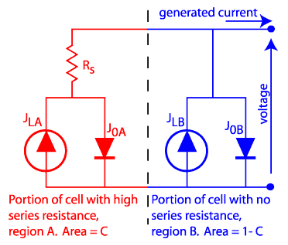
\includegraphics[width=0.5\textwidth]{cell_with_varying_series_resistance.png}
    \caption{Solar Cell With Varying Series Resistances~\cite{pveducation_measurement_of_series_resistance}}
    \label{fig:cell_with_varying_series_resistance}
\end{figure}

Replication of Fébba et al's work is presented in
Appendix~\ref{appendix:parasitics_measurements}, where a custom testbed is used
to measure solar cell curves at various temperature and irradiance levels at a
broader range compared to Fébba et al ($0\si{\celsius}$ to $100\si{\celsius}$
and $0\si{\watt/\meter^2}$ to $1000\si{\watt/\meter^2}$, respectively).
Additionally, Appendix~\ref{appendix:parasitics_measurements} also discusses
methods to evaluate the resistances and their respective coefficients. The
evaluation of the effectiveness of these terms in predicting the expected
\ac{I-V} curves warrants their own subsection in
Section~\ref{sec:evaluation_of_solar_cell_models}.


\subsection{Model Summary}\label{subsec:five_param_model_summary}

To conclude this major section, we will review the components that make up the
five parameter cell model, propose an item of further exploration, and propose a
complete model function that incorporates the topics discussed.

Firstly, the five parameter cell model retains the attributes of the three
parameter cell model, being the complete form of the single diode model. It adds
two parameters, a shunt resistance \ac{RSH} and series resistance \ac{RS} that
represent ohmic losses in the solar cell, which primarily affect the knee-bend of
the resultant \ac{I-V} curve. These two parameters help reduce error in the
model around the knee-bend that cannot fully be represented by the ideality
factor. However, these additions increase the complexity of the model, and the
resultant form is an implicit equation that requires an iterative solver
approach.

Secondly, we investigate a revision to the photocurrent model to make it also a
function of the shunt and series resistance. This was obtained by evaluating the
short circuit condition of the existing model and reducing the dark current term
under appropriate conditions. We note that this new model may not work under
specific conditions, namely for concentrator solar cells or for solar cells with
inordinately large series resistance relative to their specific \ac{VOC} and
\ac{ISC} combination.

We also discuss evaluating the shunt and series resistance themselves as a
function of temperature and irradiance. We observe that these values tend to
have exponential relationships with temperature and linear relationships with
irradiance, although we require further data to validate the strength of these
correlations. We derive initial models for these parameters, and discuss
real world conditions in which they might deviate from our expectations (e.g.
partial shading).

As such, we will revisit both of these modifications to the base model in a
further section to prove or disprove their veracity and usefulness to the
overall model.

Finally, we incorporate these changes into the complete function defined in the
previous section. This is presented as Equation~\ref{eq:cell_output_current_6}
(\ac{ISC}, \ac{VOC}, \ac{RS}, \ac{RSH}, and \ac{VT} abstracted out for clarity
and brevity).

\todo{Reformat this equation}
\begin{equation}
    \begin{split}
        I_L(V_L, G, T_C) &= I_{PV}(G, T_C, R_S, R_{SH}) - I_D(V_L, G, T_C, R_S) - I_{SH}(R_S, R_{SH}) \\
        & = I_{SC}(G, T_C)\frac{R_S + R_{SH}}{R_{SH}} - I_0(G, T_C)[\exp(\frac{V_L + I_L R_S}{V_T(T_C)}) - 1] - \frac{V_L + I_L R_S}{R_{SH}} \\
        & = I_{SC}(G, T_C)\frac{R_S + R_{SH}}{R_{SH}} - I_{SC}(G, T_C)\frac{\exp(\frac{V_L + I_L R_S}{V_T(T_C)}) - 1}{\exp(\frac{V_{OC}(G, T_C)}{V_T(T_C)}) - 1} - \frac{V_L + I_L R_S}{R_{SH}} \\
        & = I_{SC}(G, T_C)[\frac{R_S + R_{SH}}{R_{SH}} + \frac{1 - \exp(\frac{V_L + I_L R_S}{V_T(T_C)})}{1 - \exp(\frac{V_{OC}(G, T_C)}{V_T(T_C)})}] - \frac{V_L + I_L R_S}{R_{SH}}
    \end{split}
    \equnit{\si{\ampere}}
    \label{eq:cell_output_current_6}
\end{equation}

\todo[inline]{See \url{https://www.desmos.com/calculator/yp0rhmabkz} to play
around with the complete three parameter solar cell model. Add as a figure later
on compared to experimental data.}
